\documentclass[simplex.tex]{subfiles}
% NO NEED TO INPUT PREAMBLES HERE
% packages are inherited; you can compile this on its own
\definecolor{jgreen}{HTML}{197300}
\definecolor{jblue}{HTML}{0000cd}
\definecolor{jred}{HTML}{cc0000}

\begin{document}

\subsection{meda}

Matrix Exploratory Data Analysis (meda) is a package being developed to
allow for easy generation of modern summary statistics effective for
high-dimensional data analysis. 

\begin{compactitem}
  \item Source code: \href{https://github.com/neurodata/meda}{https://github.com/neurodata/meda}
  \item Example output generated from Fisher's Iris data is here:
    \href{http://docs.neurodata.io/meda}{http://docs.neurodata.io/meda}
\end{compactitem}

The goal of this package is to realize the following checklist: Given a new set of n samples of vectors in $\mathbb{R}^d$

\begin{compactenum}
  \item histogram of feature types (binary, integer, non-negative, character, string etc.)
  \item \# NaNs per row? Per column? Infs per row? Per column? "Zero" variance rows? columns?
  \item Heat map of raw data that fits on screen (k-means++ to select 1000 samples, CUR to select 100 dimensions)
  \item 1st moment statistics
  \begin{compactenum}
    \item mean (line plot + heatmap)
    \item median (line plot + heatmap)
  \end{compactenum}
  \item 2nd moment statistics
  \begin{compactenum}
    \item correlation matrix (heatmap)
    \item matrix of energy distances (heatmap)
  \end{compactenum}
  \item density estimate
  \begin{compactenum}
    \item 1D marginals (Violin + jittered scatter plot of each dimension,  if n > 1000 or d>10, density heatmaps)
    \item 2D marginals (Pairs plots for top ~8 dimensions, if n*d>8000, 2D heatmaps)
  \end{compactenum}
  \item Outlier plot 
  \item cluster analysis (IDT++)
  \begin{compactenum}
    \item BIC curves
    \item mean line plot
    \item covariance matrix heatmaps
  \end{compactenum}
  \item spectral analysis
  \begin{compactenum}
    \item cumulative variance (with elbows) of data matrix
    \item eigenvectors (pairs plot + heatmap)
  \end{compactenum}
\end{compactenum}


\begin{compactitem}
\item To rescale the data in case of differently scaled features, we will implement the following options: 
\begin{compactitem}
  \item raw
  \item linear options
  \begin{compactitem}
    \item linear squash between 0 \& 1
    \item mean subtract and standard deviation divide
    \item median subtract and median absolute deviation divide
    \item make unit norm
  \end{compactitem}
  \item nonlinear
  \begin{compactitem}
    \item rank
    \item sigmoid squash
  \end{compactitem}
\end{compactitem}

\item To robustify in the face of outliers, we will utilize
 \href{http://projecteuclid.org/euclid.bj/1438777595}{Geometric median and robust estimation in Banach spaces} 

\item { if features have categories}
\begin{compactenum}
  \item sort by category
  \item color code labels by category
\end{compactenum}

\item { if points have categories}: 
   label points in scatter plots by symbol
\end{compactitem}

\vspace{12pt}

For point 6 (a) in the above checklist we have developed functionality
in \verb+meda+ to plot 1-dimensional heatmaps.  The 1D heatmap is
a different representation of a histogram, using color to denote count
instead of bin height, see figure~\ref{fig:meda}.

\begin{figure}[!h]
\begin{cframed}
\centering
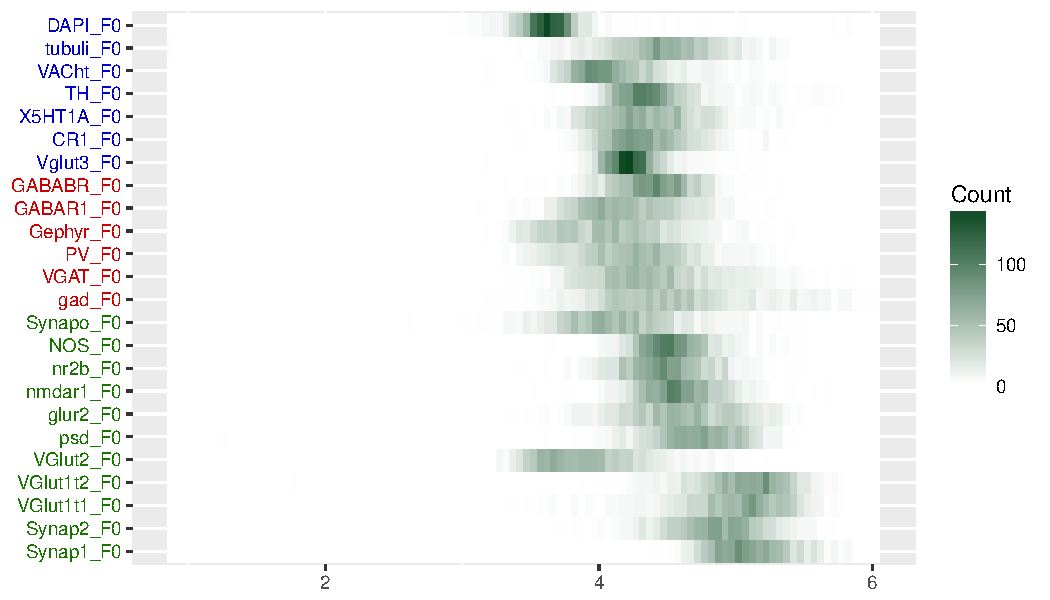
\includegraphics[width=0.95\textwidth]{../../figs/201701-meda-1dheat.pdf}
\caption{A one dimensional heatmap for each of the $\log_{10}$
  transformed feature columns of the Kristina15 synaptome dataset.
  Colors correspond to the count of data points falling in to each bin.
  Scott's binning streategy is used which, in this case, yields 105 bins
  of equal width $w = 0.05$. 
  Label colors and groups starting from the bottom:
  \textcolor{jgreen}{Synap1\_F0 - Synapo\_F0 (green, excitatory)},
  \textcolor{jred}{gad\_F0 - GABABR\_F0 (red, inhibatory)},
  \textcolor{jblue}{Vglut3\_F0 - DAPI\_F0 (blue, other)}.
  }
\label{fig:meda}
\end{cframed}
\end{figure}


\end{document}
